\label{sec:Grundstrukturen}

Im Verlauf der konzeptionellen und inhaltlichen Ausarbeitung von \acrshort{dht} wurde deutlich, dass es einen zunehmenden Bedarf an visuellen Darstellungen der Konzepte gibt. Insbesondere bei der Gestaltung und Entwicklung von Benutzerschnittstellen gab es Defizite, die durch die angewandten Methoden nicht ausgeglichen werden konnten. Eine Lösung hierfür waren Wireframes, die in der Softwareentwicklung sehr beliebt sind. \\
Wireframes sind besonders geeignet, um Weboberflächen zu visualisieren, da sie schnell erstellt und angepasst werden können und jedem ein gutes Verständnis vermitteln können. Ein weiterer Vorteil besteht darin, dass Kunden zeitnah die ersten Designkonzepte präsentiert werden können und ihr Feedback in frühen Entwicklungsphasen einfließen kann. \\
Die Erstellung von Wireframes erfordert gleichzeitig eine Auseinandersetzung mit dem Aufbau und der Konzeption der Website. Folglich werden in diesem Kapitel zunächst die Grundlagen für Seitenstrukturen (\ref{sec:seitenstruktur}) und Layouts (\ref{sec:layout}) erarbeitet, bevor Wireframes (\ref{sec:wireframes}) näher eingegangen werden.

\subsection{Grundlagen Seitenstruktur}
\label{sec:seitenstruktur}

Bei der Erstellung einer Website ist es daher wichtig, die Seitenstruktur im Vorfeld zu planen und zu entwerfen. Eine klare Seitenstruktur ermöglicht es den Nutzern, sich auf der Website zurechtzufinden und schnell die gewünschten Informationen zu finden.

\begin{figure}[!htb]
    \centering
    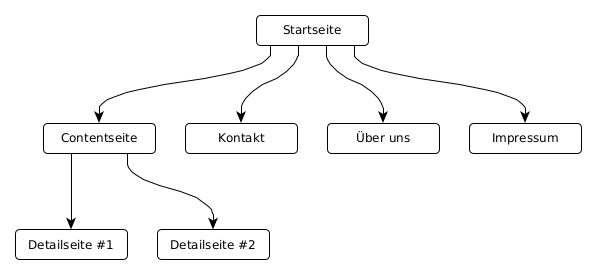
\includegraphics[scale=0.55]{figures/jan/Wire_Hierarchie.png}
    \caption[Seitenstruktur einer Website]{Seitenstruktur einer Website}
    \label{fig:seitenstruktur}
\end{figure}

Abbildung \ref{fig:seitenstruktur} zeigt beispielhaft die Seitenstruktur einer Website, bei der die Informationen thematisch aufgeteilt und auf einzelnen Seiten organisiert sind. Jede Seite hat ein klares Ziel und informiert über bestimmte Inhalte. Darüber hinaus gibt es auf jeder Website eine Reihe von Kernseiten, die oft zu finden sind, wie beispielsweise die Startseite, Kontaktseite, Landingpage, Content- sowie Detailseiten.

Die Startseite einer Website, auch als Homepage bekannt, bildet den Startpunkt und die zentrale Anlaufstelle für den Nutzer. Von hier aus können alle Unterseiten über entsprechende Verlinkungen erreicht werden. \\
Die Landingpage ist die erste Seite, die ein Nutzer sieht, wenn er über einen externen Link auf die Website gelangt und eine Sitzung startet. Sie wird häufig im Rahmen von Marketingmaßnahmen eingesetzt, um den Nutzer von den Angeboten der Website zu überzeugen und zu weiteren Schritten zu animieren. \\
Die Contentseite bietet einen Überblick über die verfügbaren Inhalte und verlinkt auf die zugehörige Detailseite, auf der die Inhalte ausführlich dargestellt werden. Es ist wichtig, dass die Contentseite übersichtlich gestaltet ist und dem Nutzer einen schnellen Zugang zu den relevanten Informationen bietet.

Wie aus der Beschreibung der verschiedenen Seitentypen hervorgeht, werden diese in unterschiedlicher Reihenfolge oder zu unterschiedlichen Zeitpunkten aufgerufen. Dies führt zu einer gewissen Hierarchie zwischen den Seiten. Ob diese Hierarchie flach oder tief ist, hängt von der Navigationsstruktur ab. Im Allgemeinen wird empfohlen, flache Seitenhierarchien zu verwenden, um eine bessere Orientierung für den Nutzer zu gewährleisten. \\
Die einzelnen Seiten einer Website unterscheiden sich in der Regel nicht vollständig voneinander, sondern folgen einem gleichbleibenden Aufbau. Dieses Grundgerüst einer Seite besteht oft aus einer Kopf- und Fußleiste sowie einem Inhaltsbereich (siehe Abb. \ref{fig:Grundgeruest}). Die Kopf- und Fußleiste sind üblicherweise auf allen Seiten gleich gestaltet, um eine konsistente Nutzererfahrung zu gewährleisten.

Der Kopfbereich einer Webseite ist ein wichtiger Bestandteil des Layouts und befindet sich im obersten Teil der Seite. Er umfasst üblicherweise das Logo, die Haupt- und Metanavigation und wird oft auch als Header bezeichnet. \\
Das Logo dient als visuelles Erkennungsmerkmal und soll das Unternehmen oder die Marke repräsentieren. Die Hauptnavigation ermöglicht eine strukturierte Übersicht über die verfügbaren Inhalte und ist entscheidend für eine gute Navigation auf der Webseite. Daher wird sie oft auffällig im oberen Bereich platziert. Die Metanavigation bietet ergänzende Serviceinhalte wie zum Beispiel Account-Einstellungen und ist getrennt von den Hauptthemen aufgeführt. \\

\begin{figure}[!htb]
    \centering
    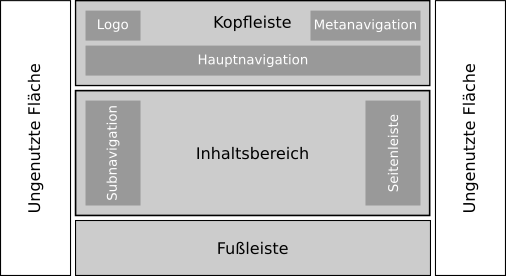
\includegraphics[scale=0.8]{figures/jan/Wire_Areas.png}
    \caption[Grundgerüst einer Website]{Grundgerüst einer Website}
    \label{fig:Grundgeruest}
\end{figure}

Der Inhaltsbereich befindet sich direkt unter dem Kopfbereich und enthält die zu vermittelnden Inhalte. Je nach Bedarf kann er entweder nur die reinen Inhalte oder auch eine Subnavigation auf der linken Seite sowie eine Seitenleiste für weiterführende Inhalte auf der rechten Seite enthalten. Die zentralen Inhalte werden zwischen den Leisten im Inhaltsbereich platziert und in der Regel nach Wichtigkeit absteigend sortiert dargestellt. \\
Die untere Begrenzung einer Webseite wird üblicherweise durch die Fußleiste gebildet. Hier finden sich häufig Basisinformationen zur Seite, ergänzende Inhalte sowie gegebenenfalls weitere Navigationsmöglichkeiten. \\
Die Seitenbereiche werden dabei von einem umgebenden Block eingerahmt, der die ungenutzte Fläche der Website darstellt.

\subsection{Grundlagen Layout}
\label{sec:layout}

\subsubsection{Rastersystem}

Um die ersten Skizzen in ein stimmiges Layout zu überführen, kann ein Rastersystem verwendet werden. Dabei handelt es sich um ein Netz mit Zeilen und Spalten, an denen die Inhalte ausgerichtet und schließlich im Rastersystem (siehe Abbildung \ref{fig:gridSystem}) platziert werden. Der Vorteil besteht darin, dass die Inhaltselemente und Einzelseiten in eine einheitliche Struktur gebracht werden und die Seiten dadurch zunehmend abgestimmter und harmonischer wirken. Das Raster wird lediglich für die Gestaltung verwendet und sollte für den Endnutzer möglichst unauffällig oder dezent wirken.

Die Basis eines Rastersystems ist in der Regel eine Leinwand mit festen Abmessungen. Diese Fläche wird in Spalten aufgeteilt und gegebenenfalls mit gleichbleibendem Freiraum zwischen den Spalten versehen. Je mehr Spalten man wählt, desto größer wird der gestalterische Spielraum, aber auch der Nutzen des Rastersystems nimmt ab einer gewissen Spaltenanzahl ab.
Im nächsten Schritt kann eine horizontale Unterteilung vorgenommen werden, wobei das sogenannte Baseline Grid als Grundlage dient. Das Baseline Grid setzt sich aus der Schriftgröße und dem Zeilenabstand zusammen.
Die einzelnen Spalten und Zeilen können weiterhin in Bereiche unterteilt werden, um ein modulares Rastersystem zu schaffen.
Abschließend werden die Inhalte der Website den entsprechenden Bereichen zugeordnet und am Raster ausgerichtet. Das Ziel ist, ein stimmiges Layout zu erreichen und den visuellen Eindruck der Website zu verbessern.


\begin{figure}[!htb]
    \centering
    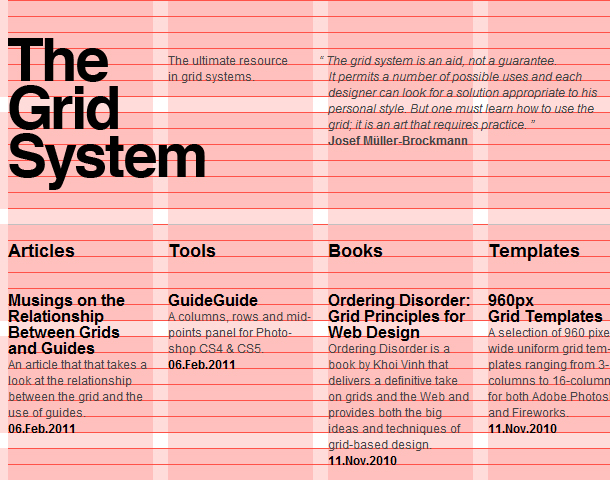
\includegraphics[width=0.6\textwidth]{figures/jan/Wire_Gridsystem.jpeg}
    \caption[Beispiel eines Rastersystems]{Beispiel eines Rastersystems \cite{gridSystem}}
    \label{fig:gridSystem}
\end{figure}

\subsubsection{Layouttypen}

Früher wurde aufgrund der begrenzten Anzahl von Endgeräten mit unterschiedlichen Auflösungen oft ein statisches Layout verwendet, das für eine gängige Auflösung optimiert war. Heute ist dieser Ansatz aufgrund der Vielzahl an Geräten mit sehr unterschiedlichen Auflösungen nicht mehr praktikabel. Es ist besonders schwierig, eine passende Auflösung zu finden, die für die meisten Geräte geeignet ist.
Deshalb geht man heutzutage nicht mehr von einer festen Breite bei der Layouterstellung aus, sondern erstellt Layouts, die sich individuell an die Auflösung des Geräts anpassen.

Das fixe Layout ist ein Layouttyp, der eine feste Breite mit festen Pixelwerten definiert. Wenn die Auflösung des Bildschirms zum Layout passt, werden alle Inhalte korrekt dargestellt. Wenn jedoch die Auflösung zu hoch ist, wird der umgebende Block der Seite unnötig groß und es entsteht viel ungenutzter Platz. Wenn die Auflösung zu niedrig ist, erscheinen horizontale Scrollbalken und die Inhalte werden abgeschnitten oder unvollständig angezeigt.


\begin{figure}[!htb]
    \centering
    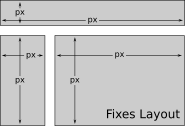
\includegraphics[scale=1.2]{figures/jan/Wire_Fixes-Layout.png}
    \hspace{0.05\textwidth}
    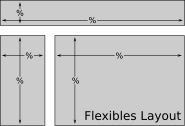
\includegraphics[scale=1.2]{figures/jan/Wire_Flexibles-Layout.png}
    \caption[Aufbau eines fixen und flexiblen Layouts]{Aufbau eines fixen und flexiblen Layouts}
    \label{fig:image}
\end{figure}

Das flexible Layout bildet das Gegenstück zum fixen Layout und zeichnet sich durch seine Fähigkeit aus, sich unmittelbar allen Veränderungen anzupassen und dabei alle vorgegebenen Größenverhältnisse beizubehalten. Im Gegensatz zum fixen Layout wird es mit relativen prozentualen Werten definiert, wodurch es sich leicht verschiedenen Varianten einer Website anpassen kann. Obwohl der reine Layouttyp selten zum Einsatz kommt, findet man häufig eine Mischform aus fixem und flexiblem Layout.

Eine weitere Layoutform ist das elastische Layout, bei dem sich die Inhalte einer Seite flexibel anpassen können. Dieser Layouttyp eignet sich besonders für Inhalte, die die volle Breite des Bildschirms ausfüllen, wie z.B. bei einer Produktpräsentation mit großformatigen Bildern und Videos. Es ist von Vorteil, wenn es nicht zu viele Inhalte gibt, da sich diese automatisch anpassen müssen, um optimal dargestellt zu werden.

Das flexible Layout bildet die Grundlage für das responsive Layout, welches die Möglichkeiten erweitert, ein passendes Layout für jedes Endgerät situationsgerecht bereitzustellen. Als Erweiterung des flexiblen Layouts verfügt das responsive Layout über sogenannte Media-Queries, die es ermöglichen, bei Überschreiten oder Unterschreiten bestimmter Schwellenwerte eine Anpassung der Ansicht zu initiieren und die Inhalte beispielsweise neu anzuordnen.

\subsection{Grundlagen Wireframes}
\label{sec:wireframes}

\subsubsection{Definition/ Inhalte}

Wireframes sind schematische Darstellungen von Inhalten und Elementen der Seitenoberfläche und dienen der Konzeptionierung in der Planungsphase. Sie ermöglichen einen groben Entwurf für die Verteilung, Anordnung und Gestaltung der Seitenelemente sowie das Herstellen von Beziehungen zwischen den Seiten.
Typischerweise sind Wireframes skizzenhafte, schwarz-weiße oder graue Abbildungen, bei denen die einzelnen Bestandteile der Seite durch einfache geometrische Formen verdeutlicht werden. Design, Farben, Schrift und Bilder sind hierbei nicht Teil der Methode. Das fertige Wireframe gibt einen Überblick über die Platzierung der Informationsinhalte, die Struktur und Navigation der Seite sowie die Interaktionselemente, mit denen der Nutzer interagiert.
Ausgearbeitete Wireframes bilden die Grundlage für die visuelle und funktionale Detaillierung des Produkts. Anschließende Schritte können beispielsweise das Erstellen von Mockups oder Prototypen sein, welche als weitere visuelle Methoden in Kapitel \ref{sec:Abgrenzung} erläutert werden.


\subsubsection{Arten}

Wireframes werden allgemein in Low-Fidelity- und High-Fidelity-Wireframes unterschieden. Bei den \acrfull{lfw} liegt der Fokus allein auf dem funktionalen Design. Die Seitenschemas werden mit einfachen Formen und ohne konkrete Inhalte erstellt. Die \acrfull{hfw} stellen hingegen die nächste Entwicklungsstufe für die Ausarbeitung des Designs dar. Hier kommen zunehmend mehr Designkomponenten wie Farben, Typographie, Abstände, Icons, Text, Bilder und Grafiken zum Einsatz. Dabei werden auch reale Textlängen und Größenverhältnisse der Elemente und Inhalte berücksichtigt.

\begin{figure}[!htb]
    \centering
    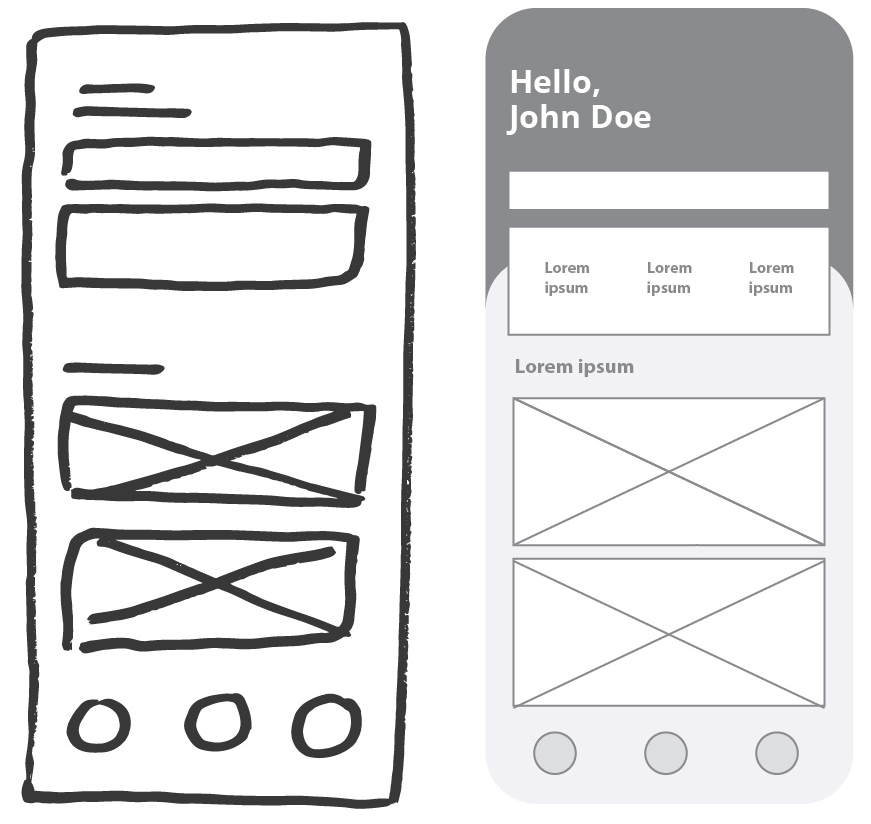
\includegraphics[scale=1]{figures/jan/Wire_Fixes-LFWvsHFW2.png}
    \caption[Beispielhafte Darstellung von \acrshort{lfw} und \acrshort{hfw}]{Beispielhafte Darstellung von \acrshort{lfw}  und \acrshort{hfw} \cite{TypeOfWireframes}}
    \label{fig:image}
\end{figure}

\subsubsection{Abgrenzung}
\label{sec:Abgrenzung}

Wireframes werden oft in Verbindung mit anderen visuellen Methoden genutzt, wie zum Beispiel Mockups und Prototypen. Diese Methoden bauen auf Wireframes auf und haben zum Ziel, das zukünftige Produkt realitätsnah darzustellen.

Mockups sind Nachbildungen oder maßstabsgerechte Modelle des Produkts und legen den Fokus auf das visuell-interaktive Design. Dabei werden die Wireframes um Elemente der Benutzeroberfläche ergänzt, jedoch sind keine funktionalen oder animierten Elemente enthalten. Mockups werden oft in der natürlichen Umgebung des Produkts, z.B. auf einem Gerätebildschirm, dargestellt, um dem Kunden ein realitätsnahes Gefühl des Erscheinungsbilds zu vermitteln.

Ein Prototyp ist ein vereinfachtes Versuchsmodell des geplanten Produkts, das auf den Ergebnissen eines Mockups aufbaut. Er wird um funktionale Elemente erweitert, um die Interaktion eines Benutzers mit dem Dienst simulieren zu können.
Ein Beispiel für einen klassischen Prototypen ist ein Klick-Dummy. Dieser bietet eine teilweise interaktive Demo einer Bedienoberfläche, die alle relevanten Merkmale des Produkts widerspiegelt. Er kann für Vorstellungen oder Testläufe genutzt werden.


\begin{figure}[!htb]
    \centering
    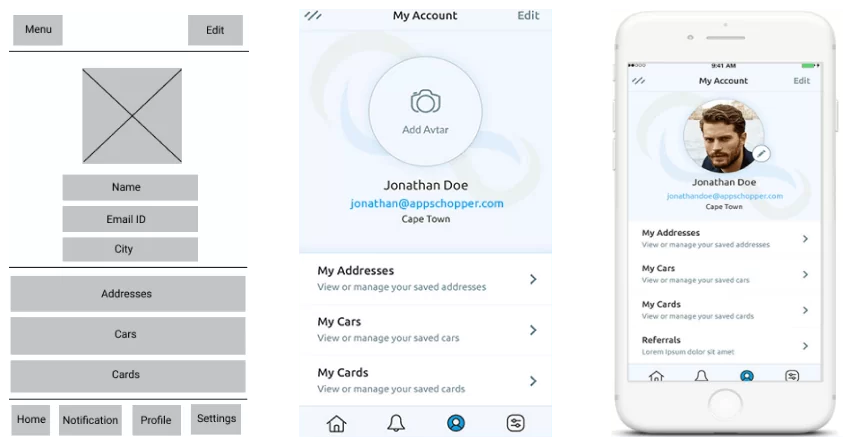
\includegraphics[scale=2]{figures/jan/Wire_Fixes-Wire-prototyp.png}
    \caption[Interationsschritte an einem Beispiel: Wireframe - Mockup - Prototyp]{Interationsschritte: Wireframe - Mockup - Prototyp \cite{LfwHfwMoc}}
    \label{fig:image}
\end{figure}

\subsection{Anwendung}
\subsubsection{Integration}

Die Wireframes wurden kontinuierlich im Projektverlauf genutzt, um die Ausgestaltung und Kommunikation der User-Stories während des Backlog Refinement zu unterstützen. Zunächst wurden in einer frühen Phase die jeweiligen User-Stories vom Product Owner erläutert und ein erster Entwurf der Wireframes erstellt. Erkenntnisse, die während der Konzeptionierung entstanden sind, wurden mit dem Product Owner besprochen und direkt in den Wireframes umgesetzt.
Während des Refinement-Prozesses dienten die Wireframes einerseits dem Product Owner zur Vorstellung und Erklärung der User-Stories und andererseits zur Präzisierung und Detaillierung der Story im Team. Die daraus gewonnenen Informationen wurden vom Product Owner in das Backlog aufgenommen und erneut in die Wireframes integriert, um sie im nächsten Refinement-Prozess zu berücksichtigen.

Die Wireframes wurden nicht nur genutzt, um die Features zu definieren und zu veranschaulichen, sondern auch während des Entwicklungsprozesses. Hier dienten sie als gestalterische Grundlage und wurden soweit wie möglich vom Entwickler implementiert.

\subsubsection{Toolauswahl}

Es gibt eine Vielzahl von Softwarelösungen, die für die Erstellung von Wireframes genutzt werden können. Diese lassen sich grob in desktop- und webbasierte Anwendungen unterteilen. Für uns war es bei der Wahl der Softwarelösung entscheidend, dass die Wireframes einfach erstellt und angepasst werden können, dass ein paralleles Arbeiten möglich ist und dass die aktuellen Entwürfe ohne zusätzlichen Aufwand geteilt werden können. Aufgrund dieser Anforderungen haben wir uns auf webbasierte Lösungen konzentriert und sind bei unserer Recherche auf Figma\footnote{Siehe \url{https://www.figma.com/}} gestoßen, das sich als passender Dienst herausgestellt hat.

\begin{figure}[!htb]
    \centering
    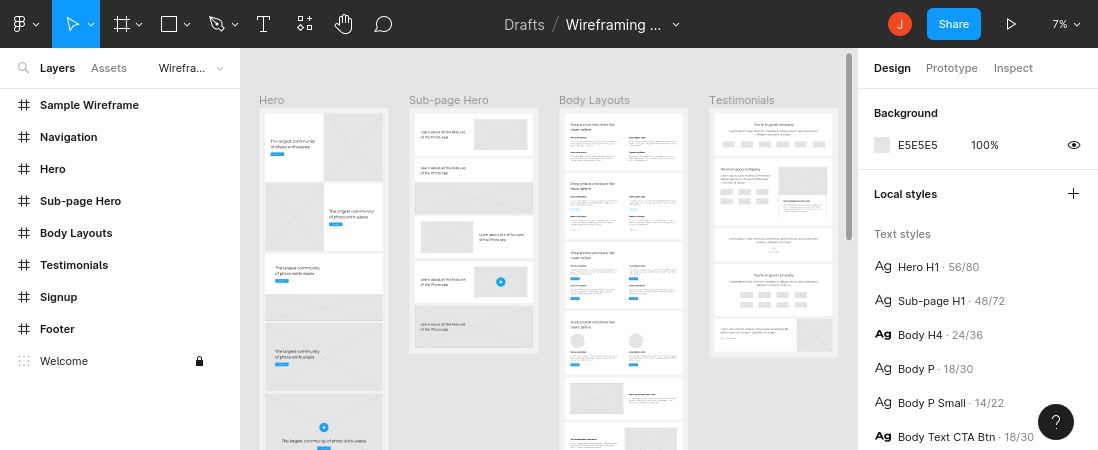
\includegraphics[width=\textwidth]{figures/jan/Wire_Figma.png}
    \caption[Figmas-Arbeitsumgebung]{Figmas-Arbeitsumgebung}
    \label{fig:figma}
\end{figure}

Figma hat sich als etablierte Onlineanwendung auf die Erstellung von Wireframes, Mockups und Prototypen spezialisiert. Als Werkzeug ist es ausgereift und unterstützt die Erstellung einfacher Wireframes durchgängig. Bei der Erstellung der Wireframes wurde sich auf die grundlegenden Funktionen von Figma beschränkt und besonders darauf geachtet, die wesentlichen Elemente zu betonen, um die Kerninhalte der Features hervorzuheben. Dazu wurden Rechtecke und Textelemente zur Gestaltung sowie Raster und Gruppierungs-Funktionen zur Orientierung und Ausrichtung der Inhaltselemente eingesetzt.

\subsubsection{Anforderungen an die Benutzerschnittstelle}

Für die Erstellung der Wireframes wurden im Vorfeld bestimmte Anforderungen festgelegt, die bei der Gestaltung berücksichtigt werden mussten. Diese Anforderungen betrafen sowohl die Gestaltung der Oberfläche als auch die technologiekonforme Umsetzung der Wireframes.

Eine wichtige Anforderung war es, die Benutzerschnittstelle -- auf engl. \acrfull{ui2} -- generationenübergreifend zu gestalten. Daraus ergaben sich folgende Anforderungen an die \acrshort{ui2}:

\begin{itemize}
    \item Eine einfache und intuitive Seitengestaltung, um Funktionsumfang und Bedienung schnell selbstständig erfassen zu können.
    \item Reduzierung der Inhalte auf das Wesentliche, um Verwirrungen und Ablenkungen zu vermeiden.
    \item Flache Hierarchien, um direkte Zugriffe auf die gewünschten Inhalte zu ermöglichen.
\end{itemize}

Um die Konzeptentwürfe erfolgreich umzusetzen, war es entscheidend, bei der Erstellung die verwendeten Webtechnologien zu berücksichtigen. So sollten die Umsetzungen der Entwürfe für die Entwickler ohne größere Schwierigkeiten erfolgen können. Ein weiteres Ziel bestand darin, einen hohen Grad an Wiederverwendbarkeit der Komponenten zu erreichen.

\subsubsection{Ausarbeitung der Seiten}

Als geeigneter Wireframetyp wurde ein Hybrid aus \acrshort{lfw} und \acrshort{hfw} gewählt. Die erstellten Wireframes umfassten alle typischen Layoutbereiche wie Kopf-, Inhalts- und Fußbereich, deren Inhalte in Feldern vereinfacht symbolisiert wurden. Die einzelnen Felder beinhalteten Texte, Dummy-Blöcke wie beispielsweise für Bilder sowie die zugehörigen Interaktionselemente wie Buttons und Dialoge.
Die Wireframes wurden in schlichtem Graustufen gehalten und ohne Berücksichtigung von Designelementen wie Farbe und Typografie erstellt. Für die regelmäßige Erstellung und Anordnung der Komponenten hat sich nach einigen Entwürfen die Leinwandbreite von 1160 Pixel mit einem Raster von 27x37 Pixel als vorteilhaft erwiesen.


Wireframes wurden für folgende Seiten/Dialoge erstellt:

\begin{itemize}
    \item Landingpage,
    \item Registrierung,
    \item Dashboard,
    \item Chat,
    \item Profil,
    \item Accounteinstellungen,
    \item Merkzettel und
    \item Marktplatz
\end{itemize}

erstellt.

Die Art und Detailtiefe der Ausgestaltung zeigen exemplarisch die Wireframes in Abbildung \ref{fig:Startseite} und \ref{fig:Marktplatz}.

\begin{figure}[!htb]
    \begin{minipage}[t]{0.5\textwidth}
        \includegraphics[page=2, width=1\textwidth]{figures/jan/wire_example.pdf}
        \caption[Startseite (\acrshort{dht})]{Startseite (\acrshort{dht})}
        \label{fig:Startseite}
    \end{minipage}
    \begin{minipage}[t]{0.5\textwidth}
        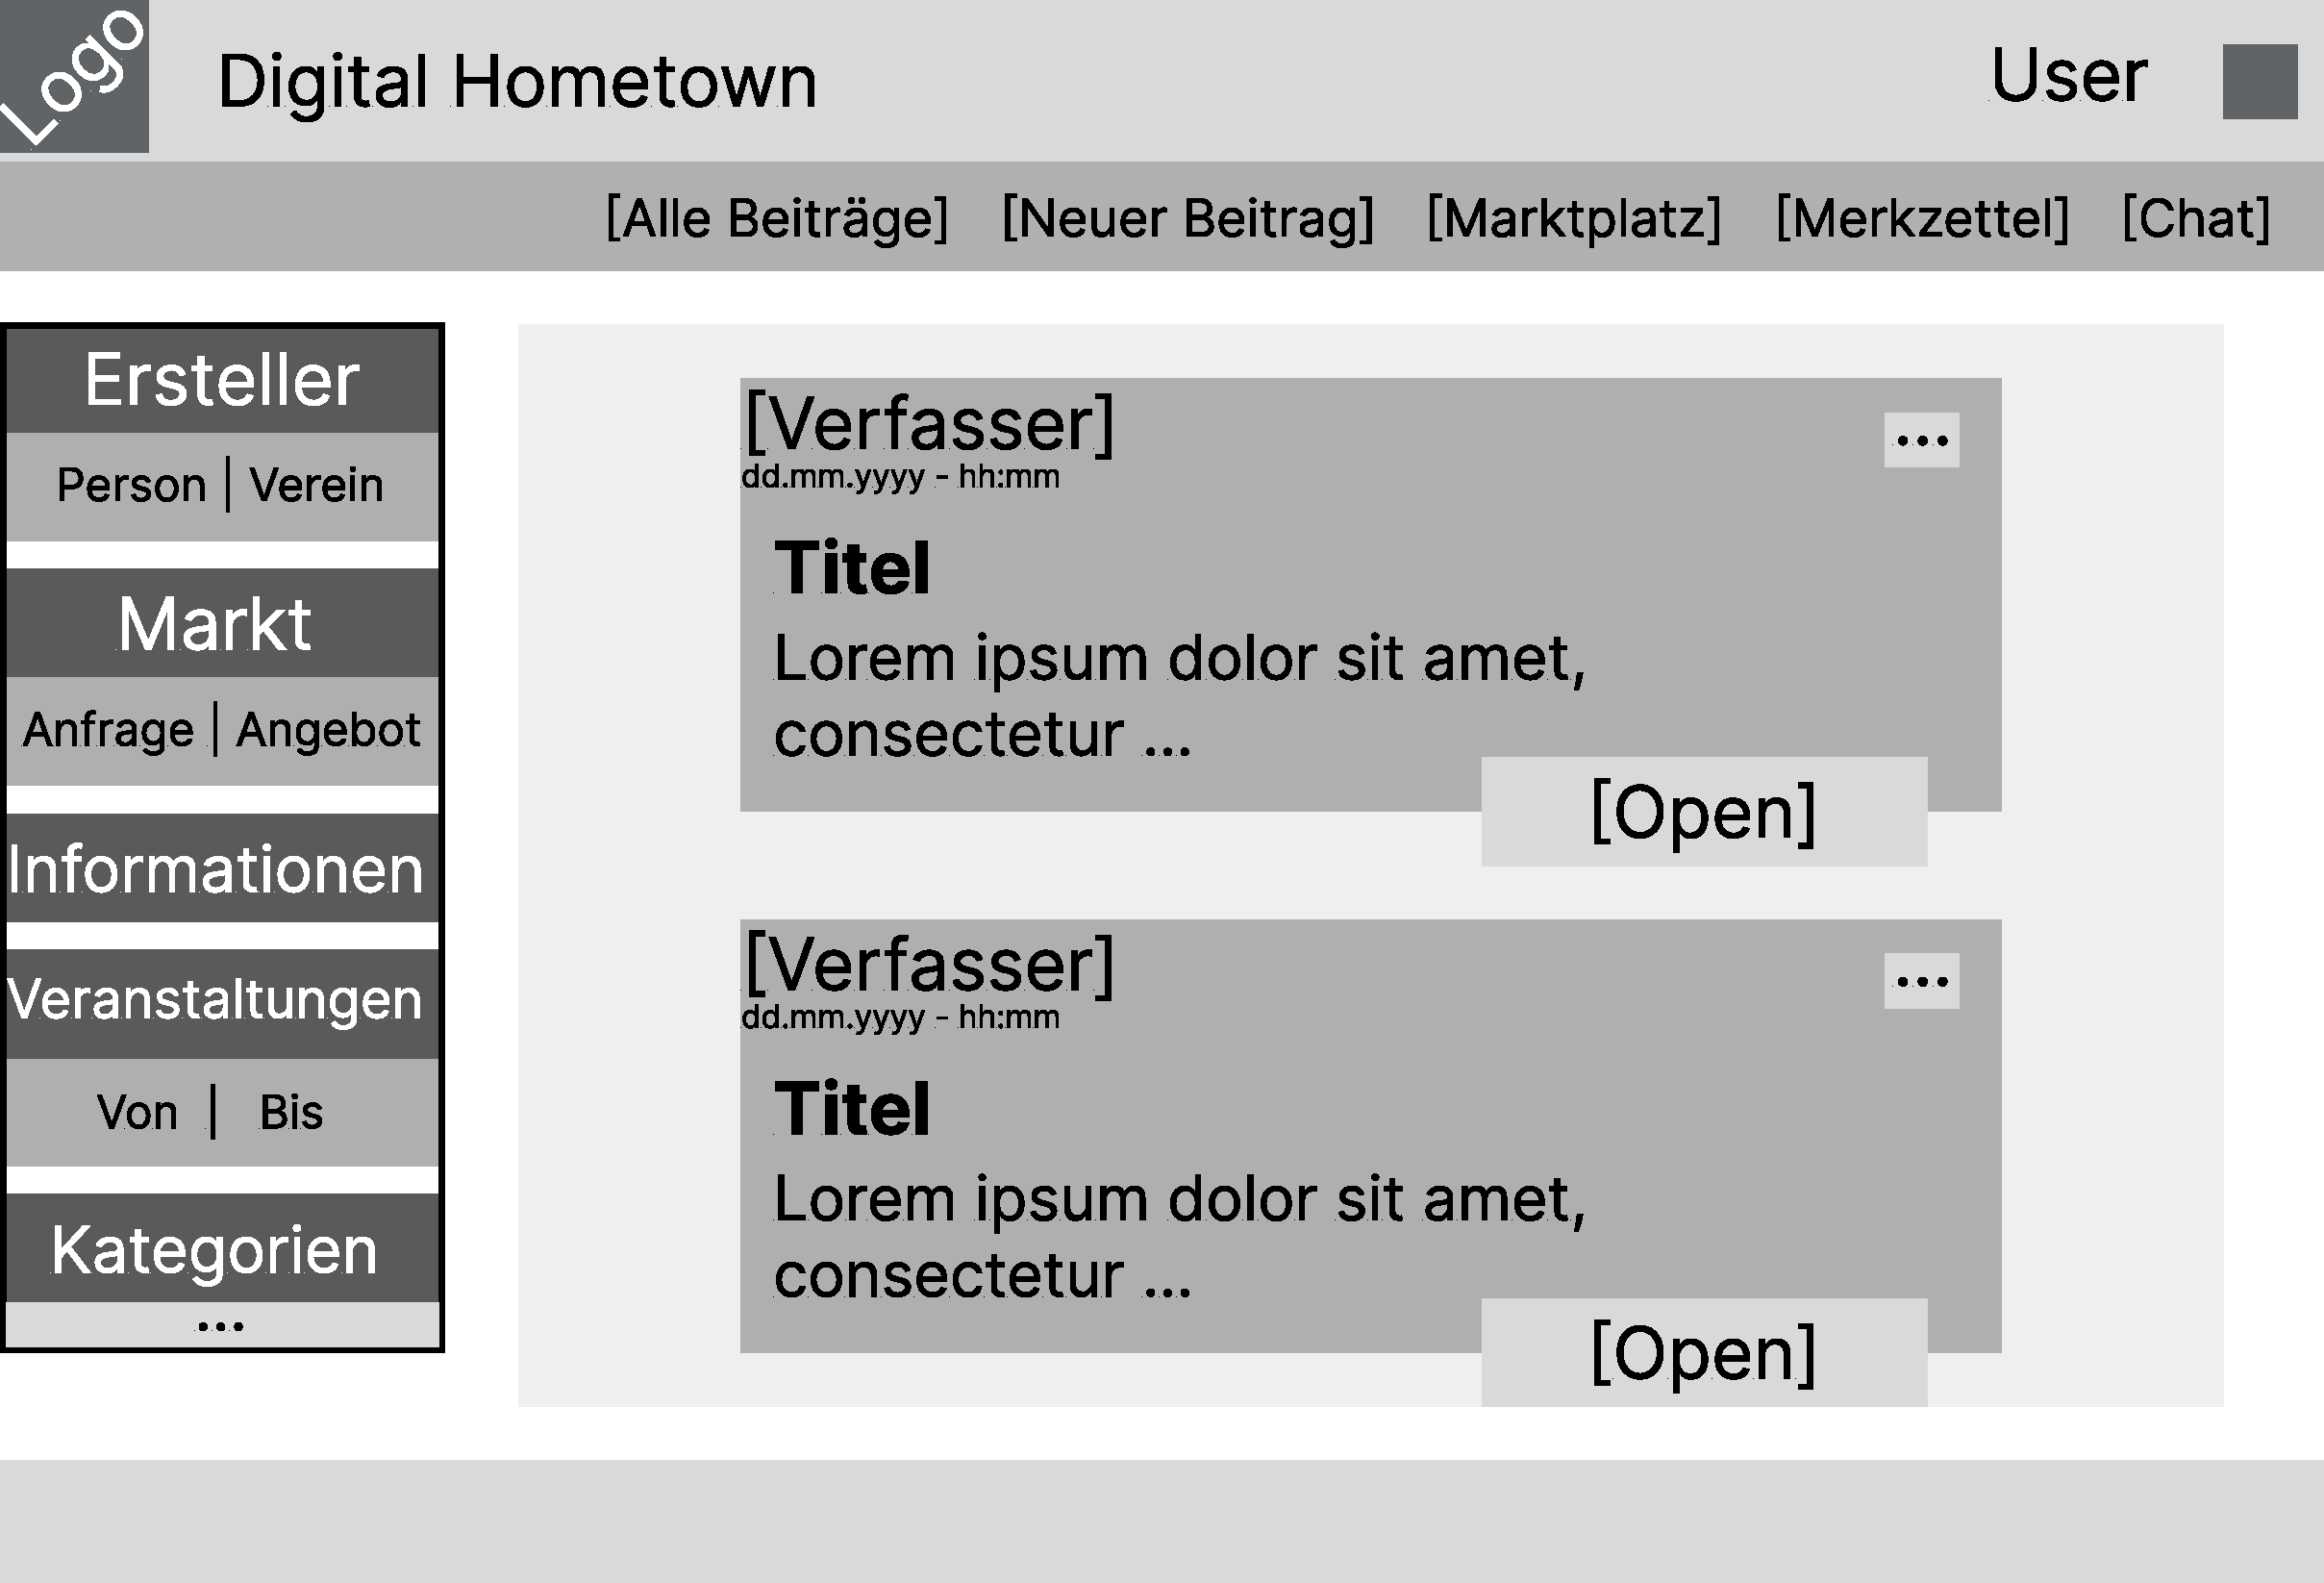
\includegraphics[page=1, width=1\textwidth]{figures/jan/wire_example.pdf}
        \caption[Marktplatz (\acrshort{dht})]{Marktplatz (\acrshort{dht})}
        \label{fig:Marktplatz}
    \end{minipage}
\end{figure}
